\documentclass[xcolor=table]{beamer}
%------------------------------------------------------------
% Theme and Appearance
%------------------------------------------------------------
\usetheme[footline=authorinstitutetitle]{Berlin} 
\setbeamertemplate{navigation symbols}{} 

% Headline with Access Code
\setbeamertemplate{headline}{
    \begin{beamercolorbox}[wd=\paperwidth,ht=2.5ex,dp=1ex,right]{section in head/foot}
        \usebeamerfont{section in head/foot}
        \hspace{0.5cm}
        \ifnum\insertframenumber<30
            \raisebox{-1pt}[0pt][0pt]{\normalsize\textbf{Attendance Code: 123456}}
        \fi
        \hspace{0.5cm}
    \end{beamercolorbox}
}
% Footline with page numbers
\setbeamertemplate{footline}{
    \leavevmode%
    \hbox{%
        \begin{beamercolorbox}[wd=.333333\paperwidth,ht=2.25ex,dp=1ex,left]{author in head/foot}%
            \usebeamerfont{author in head/foot}\hspace*{0.5em}\insertshortauthor
        \end{beamercolorbox}%
        \begin{beamercolorbox}[wd=.333333\paperwidth,ht=2.25ex,dp=1ex,center]{title in head/foot}%
            \usebeamerfont{title in head/foot}\insertshorttitle
        \end{beamercolorbox}%
        \begin{beamercolorbox}[wd=.333333\paperwidth,ht=2.25ex,dp=1ex,right]{date in head/foot}%
            \usebeamerfont{date in head/foot}\insertshortdate{}\hspace*{2em}
            \insertframenumber{} / \inserttotalframenumber\hspace*{2ex} 
        \end{beamercolorbox}}%
    \vskip0pt%
}
\usepackage[utf8]{inputenc}
\usepackage[table]{xcolor}
\usepackage{colortbl}
\usepackage{minted}
\usepackage{lmodern}
\usepackage{tgheros}
\usepackage{hyperref}
\usepackage{graphicx}
\usepackage{tikz}
\usetikzlibrary{shapes, arrows, positioning, shadows, fit, calc}

\renewcommand*\familydefault{\sfdefault}

% Agenda at the start of every section
\AtBeginSection[]
{
    \begin{frame}
        \frametitle{Agenda}
        \tableofcontents[currentsection]
    \end{frame}
}

%------------------------------------------------------------
% Title Page Information
%------------------------------------------------------------
\title[CMP9134 - Week 3]{Software Requirements \& Design Constraints}
\subtitle{CMP9134: Software Engineering}
\author[Francesco Del Duchetto]{Dr Francesco Del Duchetto\\Lecturer in Robotics and Autonomous Systems}
\institute[University of Lincoln]{University of Lincoln}
\date{20 February 2026}

%------------------------------------------------------------
\begin{document}

%--- TITLE FRAME ---
\begin{frame}
    \titlepage
\end{frame}

%--- AGENDA FRAME ---
\begin{frame}
    \frametitle{Today's Agenda}
    \tableofcontents
\end{frame}

\begin{frame}
    \frametitle{Today's Learning Objectives}
    By the end of this lecture, you should be able to:
    \begin{enumerate}
        \item \textbf{Define} the purpose of Software Requirements Engineering and distinguish between Functional and Non-Functional Requirements (NFRs).
        \item \textbf{Recognise} Legal, Ethical, Professional, and Social Issues (LEPSI) not as abstract concepts, but as strict design constraints and NFRs.
        \item \textbf{Identify} how regulatory compliance (e.g., GDPR), privacy by design, and accessibility (e.g., WCAG) dictate software architecture choices.
        \item \textbf{Apply} Agile methodologies to capture LEPSI constraints using User Stories and a robust "Definition of Done" (DoD).
    \end{enumerate}
\end{frame}

%------------------------------------------------------------
\section{What is Software Requirements Engineering?}
%------------------------------------------------------------


\begin{frame}
    \frametitle{What are Requirements?}
    \begin{block}{Definition}
        Software Requirements Engineering is the process of identifying, documenting, and maintaining software requirements.
    \end{block}
    \vspace{0.3cm}
    Requirements describe \textbf{how a software system should behave} or the \textbf{attributes it must have}.
    \begin{itemize}
        \item They ensure developers and stakeholders share a common understanding of what the software should do.
        \item \textit{A project without clear requirements is guaranteed to fail.}
    \end{itemize}
    \vspace{0.3cm}
    
    \begin{center}
        
    \end{center}
\end{frame}

\begin{frame}
    \centering
        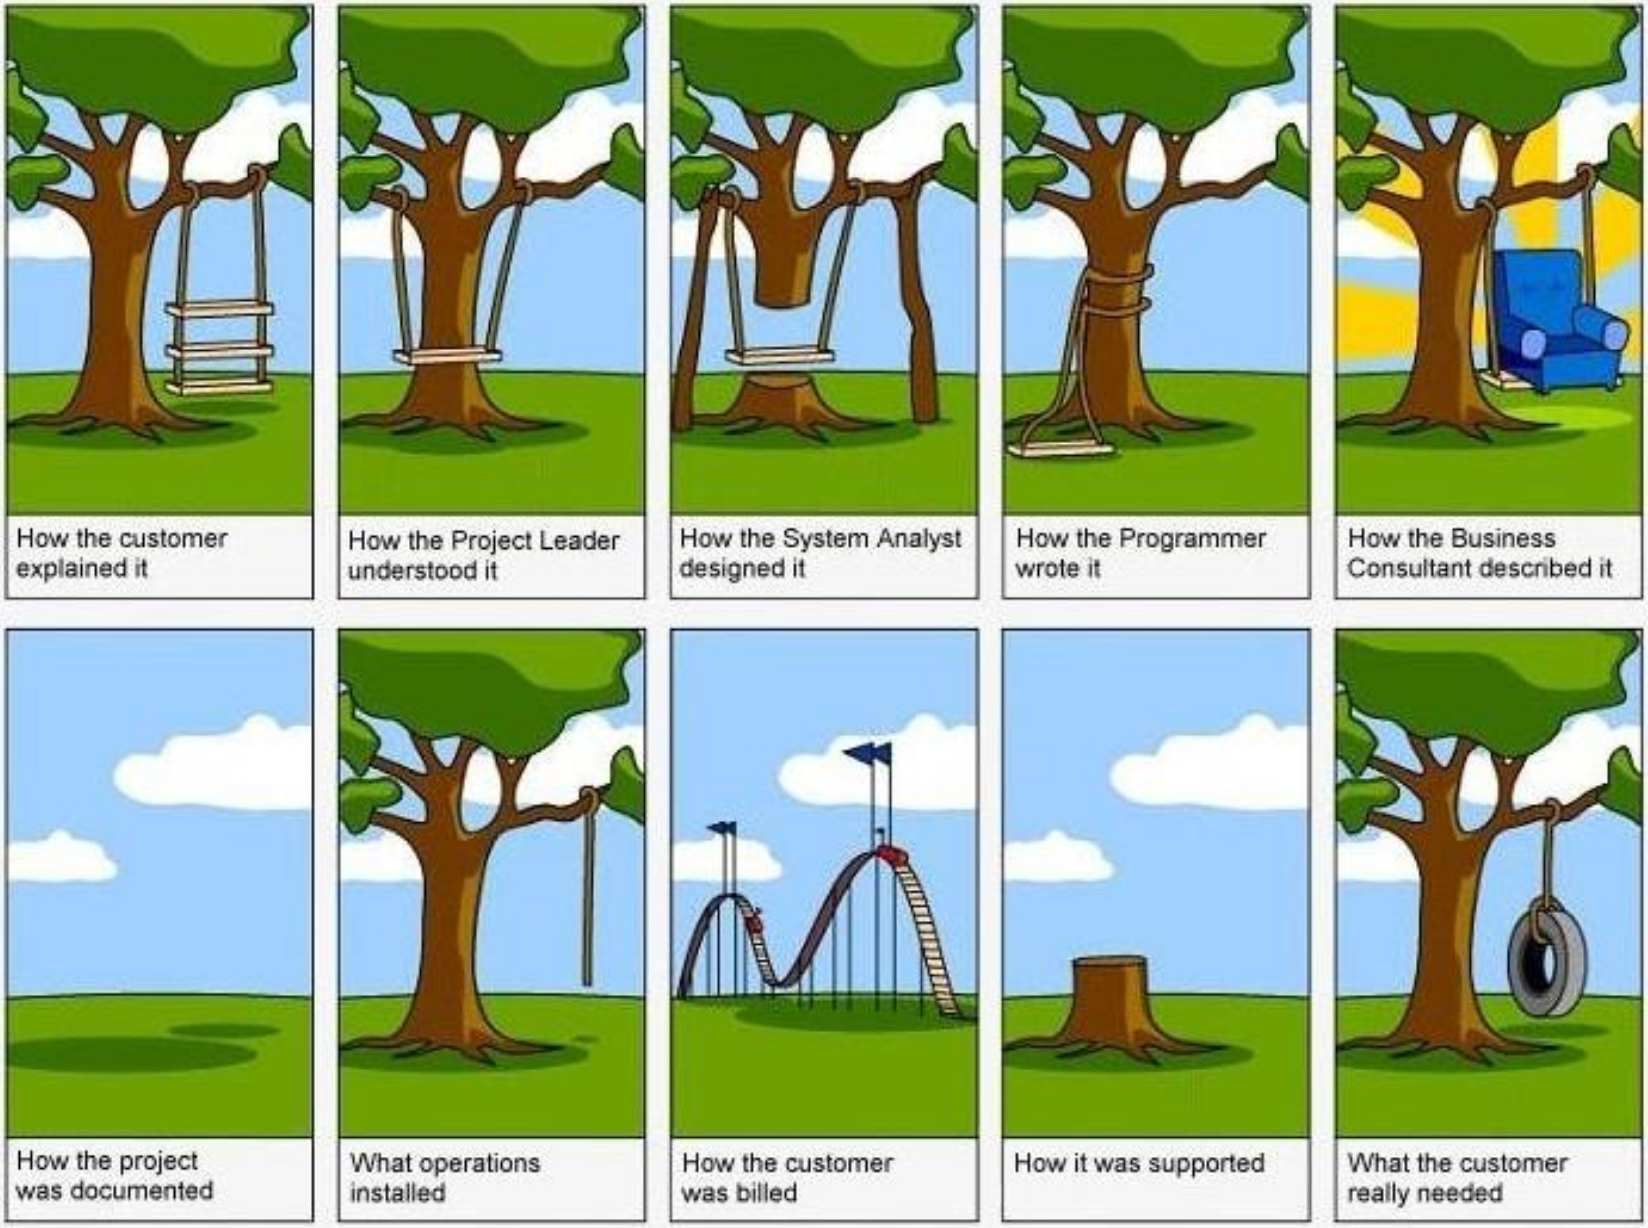
\includegraphics[width=\textwidth]{imgs/image.png}

\end{frame}

\begin{frame}[fragile]
    \frametitle{Functional vs. Non-Functional}
    \begin{columns}
        \column{0.5\textwidth}
        \begin{alertblock}{Functional Requirements}
            \textbf{What the system should DO.}
            \begin{itemize}
                \item Specific functions, commands, data processing.
                \item E.g., "The system shall allow the user to log in."
                \item E.g., "The robot must accept target coordinates."
            \end{itemize}
        \end{alertblock}
        
        \column{0.5\textwidth}
        \begin{exampleblock}{Non-Functional Requirements}
            \textbf{HOW the system should do it.}
            \begin{itemize}
                \item Quality attributes, performance, security, constraints.
                \item E.g., "The system must process the login in under 2 seconds."
                \item E.g., "The robot API connection must handle dropouts."
            \end{itemize}
        \end{exampleblock}
    \end{columns}
\end{frame}

\begin{frame}
    \frametitle{Non-Functional Requirements (NFRs)}
    NFRs are often overlooked but are critical for the success of a software project.
    Non-Functional Requirements can be divided into three main types:
    \begin{itemize}
        \item \textbf{Product Requirements:} Performance, Reliability, Usability.
        \item \textbf{Organizational Requirements:} Development standards, Delivery processes.
        \item \textbf{External Requirements:} Ethical, Legislative, Accounting, Interoperability.
    \end{itemize}
\end{frame}

\begin{frame}
    \frametitle{Metrics for Non-Functional Requirements}
    % \rowcolors{2}{gray!10}{white}
    \begin{table}
        \centering
        \small
        \begin{tabular}{|p{0.3\textwidth}|p{0.6\textwidth}|}
            \hline
                    \rowcolor{blue!20}
            \textbf{Property} & \textbf{Measure} \\
            \hline
            \textbf{Speed} & Processed transactions/second, Response time \\
                    \rowcolor{gray!20}
            \textbf{Size} & Mbytes, Storage footprint \\
            \textbf{Ease of use} & Training time, Number of help frames \\
                    \rowcolor{gray!20}
            \textbf{Reliability} & Mean time to failure, Probability of unavailability \\
            \textbf{Robustness} & Time to restart after failure, Data corruption probability \\
                    \rowcolor{gray!20}
            \textbf{Portability} & Target dependent statements, Number of target systems \\
            \hline
        \end{tabular}
    \end{table}
\end{frame}

%------------------------------------------------------------
\section{LEPSI as Design Constraints}
%------------------------------------------------------------

\begin{frame}
    \frametitle{LEPSI in Design}
    \begin{alertblock}{The Developer's Trap}
        "Requirements are just the features the user asked for."
    \end{alertblock}
    \vspace{0.3cm}
    Before you write a single line of code, you must realize that \textbf{Legal, Ethical, Professional, and Social Issues (LEPSI)} are not abstract concepts—they are \textbf{Non-Functional Requirements (NFRs)}.
    
    \vspace{0.3cm}
    \begin{itemize}
        \item \textbf{Legal} $\rightarrow$ Regulatory Compliance (e.g., GDPR, CCPA).
        \item \textbf{Social} $\rightarrow$ Accessibility (e.g., WCAG).
        \item \textbf{Professional} $\rightarrow$ Ethical Data Collection \& Privacy by Design.
    \end{itemize}
\end{frame}

\begin{frame}
    \frametitle{Regulatory Compliance as a Requirement}
    Your system architecture is dictated by law.
    \begin{itemize}
        \item \textbf{GDPR (EU,UK) / CCPA (California):} Governs the protection of personal data.
        \item \textbf{Design Constraints imposed:}
        \begin{itemize}
            \item You must obtain consent before collecting data.
            \item You must implement the "Right to be Forgotten" (deletion workflows).
            \item \textit{Architecture impact:} User data cannot be permanently baked into immutable logs.
        \end{itemize}
        \item \textbf{HIPAA (US Health) / PCI DSS (Payments):} Requires strict encryption, access controls (RBAC), and vulnerability scanning.
    \end{itemize}
\end{frame}

\begin{frame}
    \frametitle{Privacy \& Cybersecurity by Design}
    \textbf{Privacy} is protecting personal information. \textbf{Security} is protecting the systems from unauthorized access.
    
    \vspace{0.3cm}
    \textbf{How to map these to Requirements:}
    \begin{itemize}
        \item \textit{Req 1:} "The system must encrypt all user passwords using Bcrypt." (Security)
        \item \textit{Req 2:} "The system shall only collect telemetry data strictly necessary for the mission." (Privacy/Data Minimisation)
        \item \textit{Req 3:} "The system must feature Role-Based Access Control (RBAC) to separate 'Viewers' from 'Commanders'." (Security Constraint).
    \end{itemize}
\end{frame}

\begin{frame}[fragile]
    \frametitle{Accessibility as a Requirement (WCAG)}
    Accessibility ensures software is usable by all people, including those with disabilities. The W3C defines \textbf{POUR} principles:
    
    \vspace{0.3cm}
    \begin{center}
    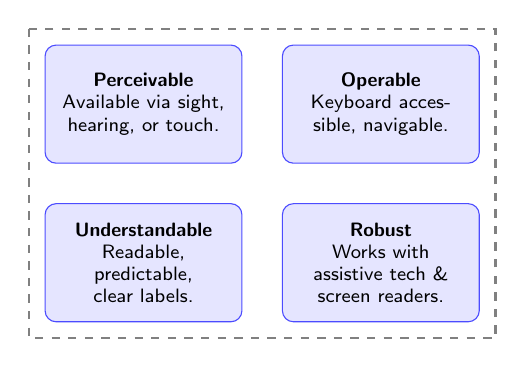
\begin{tikzpicture}[
        node distance=0.5cm and 0.5cm,
        box/.style={rectangle, draw=blue!70, fill=blue!10, rounded corners, minimum width=2.5cm, minimum height=1.5cm, align=center, text width=2.2cm, font=\scriptsize}
    ]
        \node[box] (P) {\textbf{Perceivable}\\Available via sight, hearing, or touch.};
        \node[box, right=of P] (O) {\textbf{Operable}\\Keyboard accessible, navigable.};
        \node[box, below=of P] (U) {\textbf{Understandable}\\Readable, predictable, clear labels.};
        \node[box, right=of U] (R) {\textbf{Robust}\\Works with assistive tech \& screen readers.};
        
        \draw[thick, gray, dashed] ($(P.north west)+(-0.2,0.2)$) rectangle ($(R.south east)+(0.2,-0.2)$);
    \end{tikzpicture}
    \end{center}
\end{frame}

\begin{frame}
    \frametitle{Al Ethics \& Dual Use}
    If you integrate AI or build autonomous systems (like the Robot Management System in Assessment 1), new ethical constraints emerge.
    \begin{itemize}
        \item \textbf{Explainability (XAI):} Can you explain why the robot made a specific decision? (Rule-based vs Black-box models).
        \item \textbf{Safety:} What happens when network latency causes the robot to miss a "Stop" command? (Failsafes are NFRs).
        \item \textbf{Dual Use:} Could the software you are building be used for malicious purposes if hijacked?
    \end{itemize}
\end{frame}


%------------------------------------------------------------
\section{Stages of the Requirements Process}
%------------------------------------------------------------

\begin{frame}[fragile]
    \frametitle{The Requirements Engineering Process}
    The process involves several steps, including requirements elicitation, analysis, specification, and validation, to ensure that the software will perform as intended.
    \vspace{0.3cm}
    \begin{center}
    % \footnotesize
    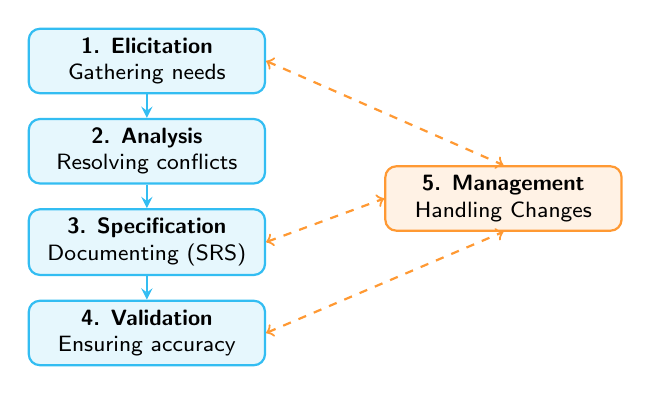
\begin{tikzpicture}[
        node distance=0.8cm,
        every node/.style={rectangle, draw=cyan!80, fill=cyan!10, thick, rounded corners, minimum width=3cm, minimum height=0.8cm, align=center, font=\footnotesize},
        arrow/.style={->, >=stealth, thick, cyan!80}
    ]
        \node (eli) {\textbf{1. Elicitation}\\Gathering needs};
        \node[below=0.3cm of eli] (ana) {\textbf{2. Analysis}\\Resolving conflicts};
        \node[below=0.3cm of ana] (spec) {\textbf{3. Specification}\\Documenting (SRS)};
        \node[below=0.3cm of spec] (val) {\textbf{4. Validation}\\Ensuring accuracy};
        
        \node[above right=-0.3cm and 1.5cm of spec, fill=orange!10, draw=orange!80] (man) {\textbf{5. Management}\\Handling Changes};
        
        \draw[arrow] (eli) -- (ana);
        \draw[arrow] (ana) -- (spec);
        \draw[arrow] (spec) -- (val);
        
        \draw[<->, dashed, orange!80, thick] (eli.east) -- (man.north);
        \draw[<->, dashed, orange!80, thick] (val.east) -- (man.south);
        \draw[<->, dashed, orange!80, thick] (spec.east) -- (man.west);
    \end{tikzpicture}
    \end{center}
\end{frame}

\begin{frame}
    \frametitle{1. Elicitation - Tools}
    This is the process of gathering requirements from stakeholders, users, and other sources. It can involve:
    \begin{itemize}
        \item \textbf{Interviews and questionnaires}.
        \item \textbf{Workshops and brainstorming} sessions.
        \item \textbf{Observation} of current systems and user behavior.
        \item Analysis of \textbf{existing documentation} and \textbf{market research}.
    \end{itemize}
\end{frame}

\begin{frame}
    \frametitle{2. Analysis - Tools}
    After gathering requirements, you need to analyze them to resolve conflicts, prioritize features, and ensure they are feasible.
    \begin{itemize}
        \item \textbf{Use Case Diagrams} to visualize interactions.
        \item \textbf{Data Flow Diagrams} to understand data movement.
        \item \textbf{Requirement Prioritization} techniques (MoSCoW, Kano).
        \item \textbf{Feasibility Analysis} to assess technical and economic viability.
    \end{itemize}
\end{frame}

\begin{frame}
    \frametitle{3. Specification - Tools}
    The Software Requirements Specification (SRS) document serves as a blueprint for development.
    \begin{block}{Key Elements of an SRS}
        \begin{enumerate}
            \item \textbf{Purpose} of the software.
            \item \textbf{Overall description} of the system.
            \item System \textbf{functionality} (Functional Req).
            \item \textbf{External Interfaces} (API connections).
            \item \textbf{Non-functional requirements} (Performance, Security).
            \item \textbf{Design Constraints} (LEPSI, Legal limits, Operating Environment).
        \end{enumerate}
    \end{block}
\end{frame}

\begin{frame}
    \frametitle{4. Validation - Tools}
    Validation ensures that the specified requirements are correct, complete, and meet stakeholder needs.
    \begin{itemize}
        \item \textbf{Reviews and Inspections} of the SRS document.
        \item \textbf{Prototyping} to gather early feedback.
        \item \textbf{Test Case Generation} to verify requirements can be tested.
        \item \textbf{Traceability Matrices} to ensure all requirements are covered by tests.
    \end{itemize}
\end{frame}

\begin{frame}
    \frametitle{5. Management - Tools}
    Managing requirements involves tracking changes, ensuring consistency, and maintaining control over the evolving scope of a project.
    \begin{itemize}
        \item \textbf{Change Request Management} to track and approve changes.
        \item \textbf{Version Control} systems to manage document versions.
        \item \textbf{Requirements Traceability} to link requirements to design and testing artifacts.
        \item \textbf{Configuration Management} to maintain system integrity across versions.
    \end{itemize}
\end{frame}


%------------------------------------------------------------
\section{Requirements in Agile Scrum}
%------------------------------------------------------------

\begin{frame}
    \frametitle{Agile Requirements: User Stories}
    In Agile, requirements are captured as \textbf{User Stories} stored in the \textbf{Product Backlog}.
    
    \vspace{0.5cm}
    \textbf{Format:}
    "As a \textbf{[User]}, I want \textbf{[Functionality]}, so that \textbf{[Benefit]}."
    
    \vspace{0.5cm}
    \textbf{Example (Applying LEPSI):}
    \textit{"As a system auditor, I want all navigation commands to be logged persistently, so that we comply with safety accountability regulations."}
\end{frame}

\begin{frame}
    \frametitle{Agile Requirements: Acceptance Criteria}
    Each User Story must be accompanied by \textbf{Acceptance Criteria} (AC) that define the conditions under which the story is considered complete.
    
    \vspace{0.3cm}
    \textbf{Purpose of AC:}
    \begin{itemize}
        \item Define clear expectations for the feature.
        \item Ensure developers and stakeholders are aligned.
        \item Provide testable conditions for validation.
    \end{itemize}
\end{frame}

\begin{frame}
    \frametitle{Definition of Done (DoD)}
    How do we know a requirement is actually met? We use a Definition of Done. 
    
    \vspace{0.3cm}
    To consider a User Story "Done", a team might agree it must pass the following checklist:
    \begin{itemize}
        \item [$\square$] \textbf{Code compiles and runs.}
        \item [$\square$] \textbf{Unit tests pass.}
        \item [$\square$] \textbf{Security scan passes} (No hardcoded passwords).
        \item [$\square$] \textbf{UI meets WCAG accessibility guidelines.}
        \item [$\square$] ...
        % \item [$\square$] \textbf{AI usage is formally logged and verified.}
    \end{itemize}
\end{frame}

\begin{frame}
    \frametitle{Practical Agile: Writing Good User Stories}
    How do you write a User Story for your Robot Management System? Avoid vague feature requests.
    
    \begin{alertblock}{Poor User Story}
        "Make the robot move." \textit{(Too vague, lacks context, no clear user or benefit).}
    \end{alertblock}

    \begin{exampleblock}{Strong User Story}
        "As a \textbf{Commander}, I want to \textbf{input X and Y coordinates into the dashboard}, so that \textbf{the robot navigates to the target location}."
    \end{exampleblock}
    
    \vspace{0.2cm}
    \textbf{Why is this better?}
    \begin{itemize}
        \item It defines \textbf{who} needs it (Commander, not a Viewer).
        \item It defines \textbf{what} the interface needs (X and Y inputs).
        \item It defines the \textbf{business value} (navigating to a target).
    \end{itemize}
\end{frame}

\begin{frame}[fragile]
    \frametitle{Acceptance Criteria vs. Definition of Done}
    While the \textbf{Definition of Done (DoD)} applies globally to \textit{every} task, \textbf{Acceptance Criteria (AC)} are specific to a \textit{single} user story.
    
    \vspace{0.3cm}
    \centering
    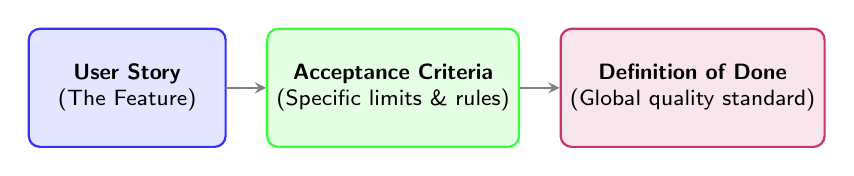
\begin{tikzpicture}[
        node distance=0.5cm,
        box/.style={rectangle, draw=black!60, fill=white, thick, rounded corners, minimum width=2.5cm, minimum height=1.5cm, align=center, font=\footnotesize},
        arrow/.style={->, >=stealth, thick, gray}
    ]
        \node[box, fill=blue!10, draw=blue!80] (story) {\textbf{User Story}\\(The Feature)};
        \node[box, fill=green!10, draw=green!80, right=of story] (ac) {\textbf{Acceptance Criteria}\\(Specific limits \& rules)};
        \node[box, fill=purple!10, draw=purple!80, right=of ac] (dod) {\textbf{Definition of Done}\\(Global quality standard)};
        
        \draw[arrow] (story) -- (ac);
        \draw[arrow] (ac) -- (dod);
    \end{tikzpicture}
    
    \vspace{0.3cm}
    \begin{itemize}
        \item \textbf{Example AC for Robot Navigation:}
        \begin{itemize}
            \item The UI must have two numeric input fields (X and Y).
            \item The system must reject negative coordinates (Error Handling).
            \item A POST request must be sent to the API's \texttt{/move} endpoint.
            \item \textbf{LEPSI Constraint:} The "Move" button must be accessible via Keyboard (WCAG).
        \end{itemize}
    \end{itemize}
\end{frame}

% \begin{frame}
%     \frametitle{Implementing this in your Workshop (Trello)}
%     How do you actually build this in your project management tools today?
    
%     \begin{enumerate}
%         \item \textbf{The Card Title:} Use the User Story format. \\
%         \textit{(e.g., "As an Auditor, I want Mission Logging...")}
%         \item \textbf{The Description (Acceptance Criteria):} Write out your specific bullet points. What exact data must be logged? (Timestamp, User ID, Command).
%         \item \textbf{The Constraints (LEPSI):} Add a note in the description about data privacy (e.g., "Ensure passwords are not saved in plaintext in this log").
%         \item \textbf{The Checklist (DoD):} Use Trello's Checklist feature to add your Definition of Done:
%         \begin{itemize}
%             \item [$\square$] Code pushed to GitHub Issue branch.
%             \item [$\square$] AI Verification Log updated in docs.
%             \item [$\square$] Acceptance Criteria tested and passed.
%         \end{itemize}
%     \end{enumerate}
% \end{frame}

%------------------------------------------------------------
\section{Next Steps}
%------------------------------------------------------------

% \begin{frame}
%     \frametitle{This Week's Lab: Requirements \& LEPSI Constraints}
%     Goal: Define the "Social/Legal" guardrails before coding the core logic for your Assessment 1 project.
    
%     \begin{itemize}
%         \item \textbf{Task 1: GDPR \& Data Privacy Audit:} Review the mission logging requirement. Identify what is PII and write a short data handling policy.
%         \item \textbf{Task 2: Definition of Done (DoD):} Create your project checklist (including AI verification logs).
%         \item \textbf{Task 3: Mocking the Requirements:} Create a JSON file to represent the API requirements to define what your frontend needs.
%         \item \textbf{Stretch Task (Distinction):} Write a paragraph outlining the "Dual Use" implications of your Ground Control Station.
%     \end{itemize}
% \end{frame}

\begin{frame}
    \frametitle{Q \& A}
    \begin{center}
        \Huge Any Questions?\\\vspace{0.5cm} 
        \normalsize fdelduchetto@lincoln.ac.uk
    \end{center}
\end{frame}

\end{document}